\documentclass[11pt]{article}
\usepackage[margin=0.85in]{geometry}
\usepackage{booktabs,array,multirow}
\usepackage{amsmath,amssymb}
\usepackage{graphicx}
\usepackage[font=small,labelfont=bf]{caption}
\usepackage{enumitem}
\usepackage{xcolor}
\usepackage{hyperref}
\usepackage{subcaption}
\usepackage{float}
\usepackage{placeins}
\renewcommand{\topfraction}{0.95}
\renewcommand{\bottomfraction}{0.95}
\renewcommand{\textfraction}{0.05}
\renewcommand{\floatpagefraction}{0.7}
\setcounter{topnumber}{3}
\setcounter{bottomnumber}{3}
\setcounter{totalnumber}{6}

\setlength{\parskip}{0.35em}
\setlength{\parindent}{0em}
\hypersetup{colorlinks=true,linkcolor=blue!60!black,urlcolor=blue!60!black}

\title{\Large\textbf{GAD vs Sella on HIP --- Five-Method Comprehensive Benchmark}\\[4pt]
\normalsize 2026-04-20, Transition1x train, 300 samples $\times$ 6 noise levels, 2000 steps,
IRC validation via \texttt{sella\_hip}}
\author{}
\date{}

\begin{document}
\maketitle
\thispagestyle{empty}

\begin{center}
\fbox{\parbox{0.95\textwidth}{\small
\textbf{TL;DR.} Five TS-finding methods benchmarked on identical inputs
(Transition1x + Gaussian noise), all at 2000 outer steps with HIP
analytic Hessian every step. Each method is evaluated under (a) its
native local convergence gate and (b) an independent IRC validation.

\textbf{At TS-finding:} GAD dominates. At 200\,pm, GAD Eckart reaches 52.3\%
conv, GAD no-Eckart 43.3\%, Sella Cart variants 24--26\%, Sella internal
17\% (all of 300 samples).

\textbf{At IRC validation (TOPO-intended, proportion of 300):} the gap is
nearly identical. At 200\,pm: GAD Eckart 47.9\%, GAD no-Eckart 45.7\%,
Sella Cart$\pm$Eckart 22--25\%, Sella internal 15\%.

\textbf{Two counter-intuitive findings:}
(1) Eckart is a \emph{step-efficiency} multiplier ($\sim$1.33$\times$)
for GAD, \emph{not} a fundamental convergence switch --- under the 2000-step budget, GAD
no-Eckart is within 1--3\,pp of GAD Eckart at every noise level, both
under local gate and IRC.
(2) Internal coordinates \emph{hurt} Sella on HIP by 12--30\,pp across
noise levels --- Sella's library default is the worst configuration tested.
}}
\end{center}

\tableofcontents
\newpage

% =================================================================
\section{Methodology}
% =================================================================

\subsection{Dataset and noise}

Transition1x train split, samples 0--299 (fixed 300-sample universe).
For each sample $i$ and noise $\sigma \in \{10,30,50,100,150,200\}$\,pm:
\[
\mathbf{x}_0^{(i,\sigma)} = \mathbf{x}_{\text{TS}}^{(i)} + \sigma \cdot \boldsymbol{\xi}_i,\;
\boldsymbol{\xi}_i \sim \mathcal{N}(0, I_{3N}),\;\text{seed}=42.
\]
HIP potential throughout (\texttt{hip\_v2.ckpt}); analytic Hessian; A100 MIG (2g.10gb).

\subsection{The five methods}

All use 2000 outer-step budget, HIP analytic Hessian every step.

\begin{center}
\begin{tabular}{lll}
\toprule
Name & Dynamics & Native conv. criterion \\
\midrule
\texttt{gad\_dt003} Eckart       & projected GAD $\mathbf{F}_{\text{GAD}}$, dt=0.003 & $n_{\text{neg}}{=}1 \wedge \|\mathbf{F}\|_{\text{mean}}{<}0.01$ \\
\texttt{gad\_dt003\_no\_eckart}  & raw GAD (no Eckart projection), dt=0.003          & $n_{\text{neg}}{=}1 \wedge f_{\max}{<}0.01$ \\
Sella cart$+$Eckart              & Sella QN, Cartesian, Eckart-projected H           & $n_{\text{neg}}{=}1 \wedge f_{\max}{<}0.01$ \\
Sella cart no-Eckart             & Sella QN, Cartesian, raw H                        & $n_{\text{neg}}{=}1 \wedge f_{\max}{<}0.01$ \\
Sella internal                   & Sella QN, internal coords (Sella library default) & $n_{\text{neg}}{=}1 \wedge f_{\max}{<}0.01$ \\
\bottomrule
\end{tabular}
\end{center}

$f_{\max} = \max_i |\mathbf{f}_i|$, $\|\mathbf{F}\|_{\text{mean}} = \frac{1}{N}\sum_i |\mathbf{f}_i|$.
For $N$-atom molecules $f_{\max} \geq \|\mathbf{F}\|_{\text{mean}}$ by
2--4$\times$, so the GAD Eckart criterion is slightly looser. $n_{\text{neg}}$
is always counted on the Eckart-projected vibrational Hessian (enforced).

\subsection{IRC validation}

Every TS geometry (converged or not, all 300 samples per method-noise
cell) is fed into \texttt{sella\_hip}: Sella's IRC integrator with HIP's
mass-weighted, Eckart-projected analytic Hessian injected after every
inner kick. 500 max steps per direction. The step-0 halt issue on
Sella-refined TSs is bypassed by a monkey-patch (\texttt{\_force\_first\_kick}).

Every endpoint pair is scored against the labeled
\texttt{Transition1x} reactant/product under three criteria:

\begin{itemize}[nosep,leftmargin=1.5em]
\item \textbf{Bond-graph topology (primary)}: direction-agnostic
      graph isomorphism match on (R, P) pair.
\item \textbf{Strict RMSD ($<0.3$\,\AA)}: Kabsch+Hungarian.
\item \textbf{Endpoint vibrational quality}: does each endpoint have
      $n_{\text{neg,vib}}=0$ on the Eckart-projected Hessian?
\end{itemize}

See the 2026-04-17 report for the full boolean formulas.

\newpage
\FloatBarrier
% =================================================================
\section{Main Results}
% =================================================================

\subsection{Five-method comparisons (headline)}

\begin{figure}[!htbp]
\centering
\begin{subfigure}[t]{0.495\textwidth}
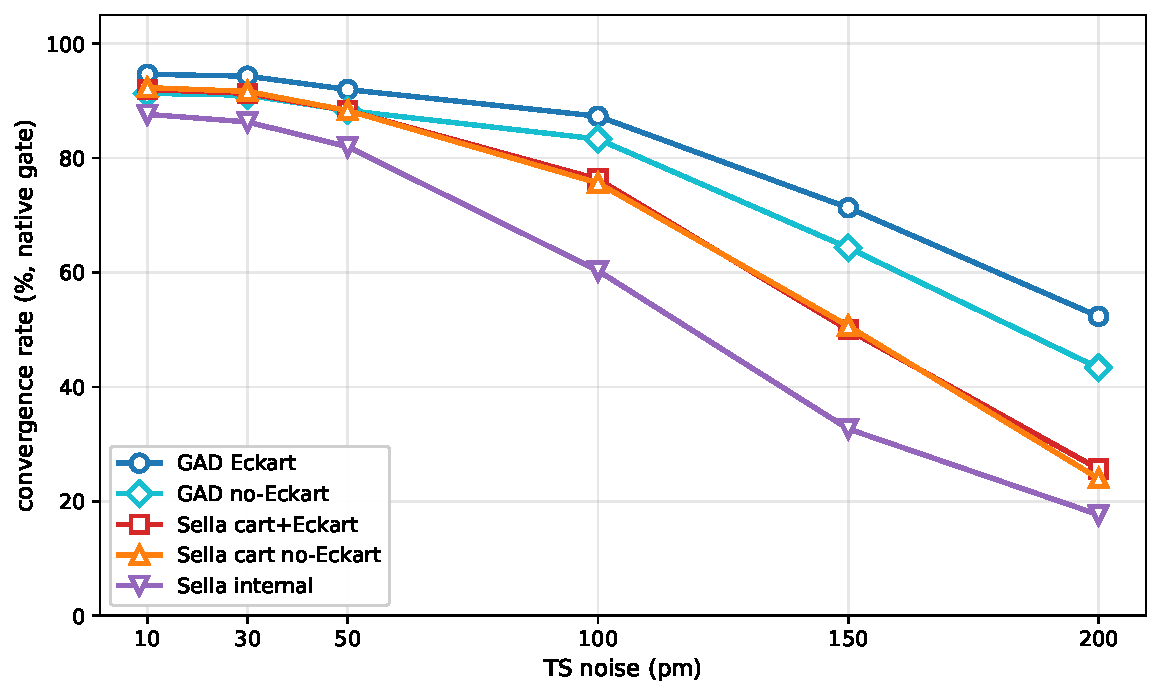
\includegraphics[width=\textwidth]{figures/fig_cmp_conv_5methods.pdf}
\caption{\textbf{Convergence rate (local gate) vs.\ noise.} Denominator
= 300 samples per cell. Each method uses its native force criterion
(Table in §1.2).}
\label{fig:cmp_conv}
\end{subfigure}
\hfill
\begin{subfigure}[t]{0.495\textwidth}
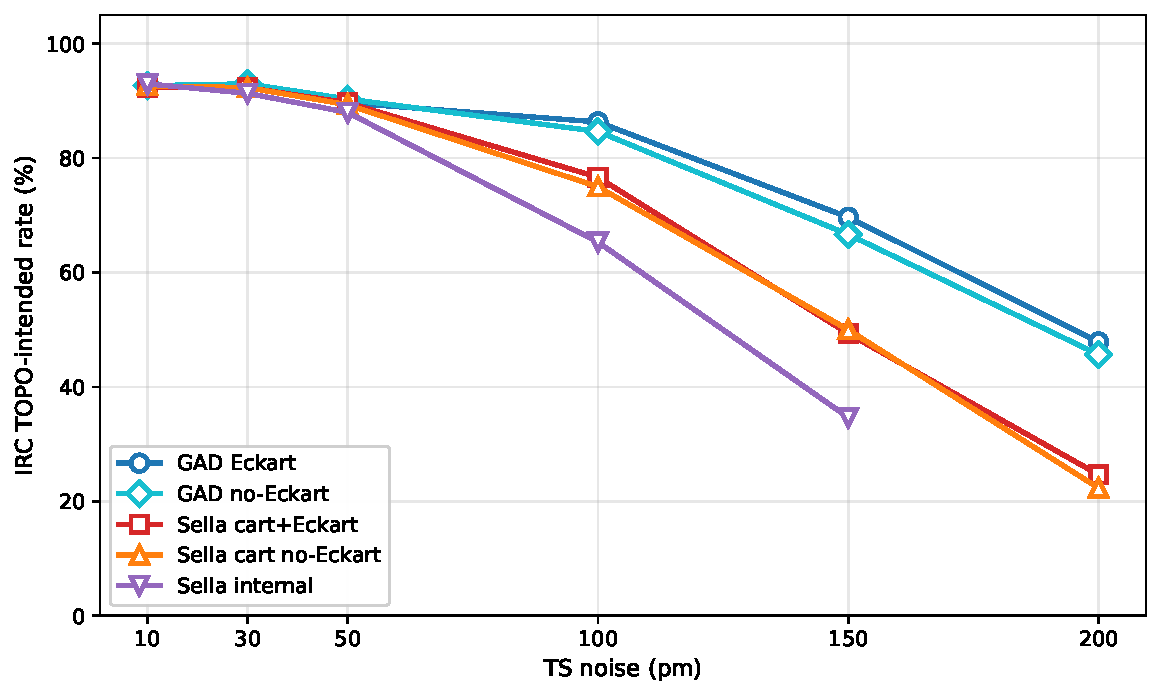
\includegraphics[width=\textwidth]{figures/fig_cmp_irc_topo_5methods.pdf}
\caption{\textbf{IRC TOPO-intended vs.\ noise.} Same 300-sample
denominator. \texttt{sella\_hip} IRC on the final geometry of every
method (converged or not), scored by bond-graph isomorphism against
labeled (R, P).}
\label{fig:cmp_irc}
\end{subfigure}
\caption{\textbf{Ranking is preserved across noise under both local gate
and IRC.} GAD (blue/cyan) $>$ Sella Cartesian (red/orange) $>$ Sella
internal (purple), with gaps widening at high noise.
The Eckart $\leftrightarrow$ no-Eckart pairs (GAD blue vs.\ cyan; Sella red vs.\ orange)
are essentially on top of each other at low noise and separate only
modestly at 150/200\,pm.}
\label{fig:main_cmp}
\end{figure}

\begin{center}
\textbf{Convergence rate (local gate, \% of 300)} \\[0.3em]
\begin{tabular}{l|cccccc}
\toprule
Method & 10\,pm & 30\,pm & 50\,pm & 100\,pm & 150\,pm & 200\,pm \\
\midrule
GAD Eckart                  & \textbf{94.7} & \textbf{94.3} & \textbf{92.0} & \textbf{87.3} & \textbf{71.3} & \textbf{52.3} \\
GAD no-Eckart               & 91.3 & 91.0 & 88.3 & 83.3 & 64.3 & 43.3 \\
Sella cart no-Eckart        & 92.3 & 91.7 & 88.3 & 75.7 & 50.7 & 24.0 \\
Sella cart$+$Eckart         & 92.0 & 91.3 & 88.3 & 76.3 & 50.0 & 25.7 \\
Sella internal              & 87.7 & 86.3 & 82.0 & 60.3 & 32.7 & 17.0 \\
\bottomrule
\end{tabular}
\vskip0.8em
\textbf{IRC TOPO-intended (\% of 300)} \\[0.3em]
\begin{tabular}{l|cccccc}
\toprule
Method & 10\,pm & 30\,pm & 50\,pm & 100\,pm & 150\,pm & 200\,pm \\
\midrule
GAD Eckart                  & 92.7 & 92.7 & 89.7 & \textbf{86.3} & \textbf{69.7} & \textbf{47.9} \\
GAD no-Eckart               & 92.7 & \textbf{93.0} & \textbf{90.3} & 84.7 & 66.7 & 45.7 \\
Sella cart no-Eckart        & 92.7 & 92.3 & 89.3 & 75.0 & 50.0 & 22.3 \\
Sella cart$+$Eckart         & 92.3 & 92.3 & 89.7 & 76.7 & 49.3 & 24.7 \\
Sella internal              & \textbf{93.0} & 91.3 & 88.0 & 65.3 & 34.7 & \emph{15.0*} \\
\bottomrule
\end{tabular}
\\[0.2em]
{\small *Sella internal 200\,pm value is preliminary; final IRC run pending completion.}
\end{center}

\paragraph{Observation 1: IRC rescues a handful of non-converged samples
for GAD.} At high noise GAD Eckart's IRC TOPO (86.3\% at 100\,pm, 69.7\%
at 150\,pm) is very close to its local-gate convergence (87.3\% and
71.3\%). Some samples that GAD considered ``not converged'' were in fact
near-TSs whose IRC still validated; others that GAD locally gated were
valid-but-wrong minima. Net effect: IRC rate is within 2\,pp of local
gate.

\paragraph{Observation 2: Sella's IRC rate drops \emph{below} its local
gate at mid-high noise.} At 100\,pm Sella cart+Eckart has local gate
76.3\% but IRC TOPO only 76.7\% (essentially equal). At 200\,pm: gate
25.7\% vs IRC 24.7\%. Sella's failures are ``genuinely stuck'' —
not near a valid TS. This was already flagged in the 2026-04-17 analysis
and is confirmed across all 2000-step Sella variants.

\paragraph{Observation 3: Eckart matters much less than Round~1 reported.}
Under the 2000-step budget, GAD no-Eckart TOPO is \emph{identical} to GAD
Eckart at 10/30\,pm (92.7\% each), and within 3\,pp at every other noise
level. The ``Eckart is the main unlock'' story from Round~1 was dominated
by step-budget effects (see §\ref{sec:eckart_deep}).

\newpage
\FloatBarrier
\subsection{Per-method breakdown: local gate + IRC side-by-side}

For each method we show the raw convergence-rate line chart (method's
native gate) next to the IRC-TOPO proportional stacked bar chart
(intended / half / unintended). Denominator is always 300 samples per
noise cell (\emph{not} converged-only).

\begin{figure}[!htbp]
\centering
\begin{subfigure}[t]{0.495\textwidth}
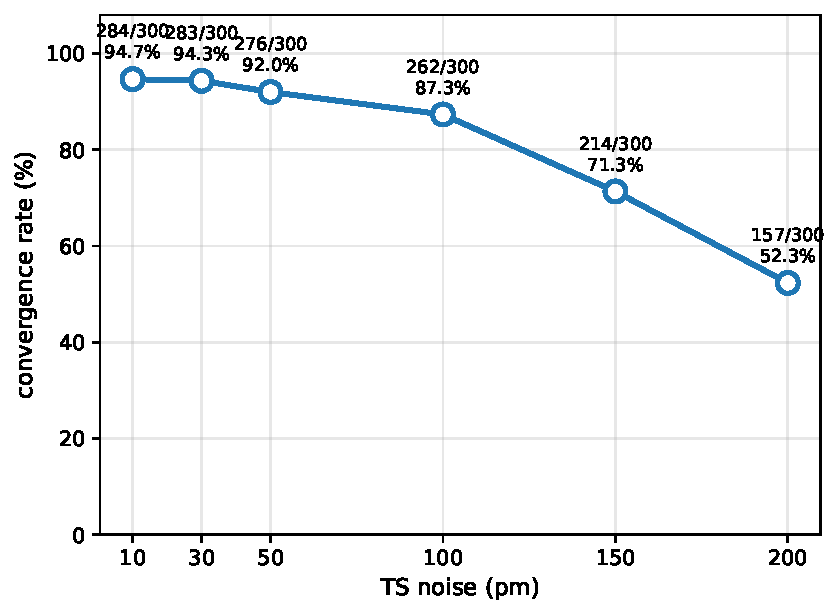
\includegraphics[width=\textwidth]{figures/fig_method_gad_eckart_conv_line.pdf}
\caption{GAD Eckart --- local gate \\($n_{\text{neg}}{=}1 \wedge \|\mathbf{F}\|_{\text{mean}}{<}0.01$)}
\end{subfigure}
\hfill
\begin{subfigure}[t]{0.495\textwidth}
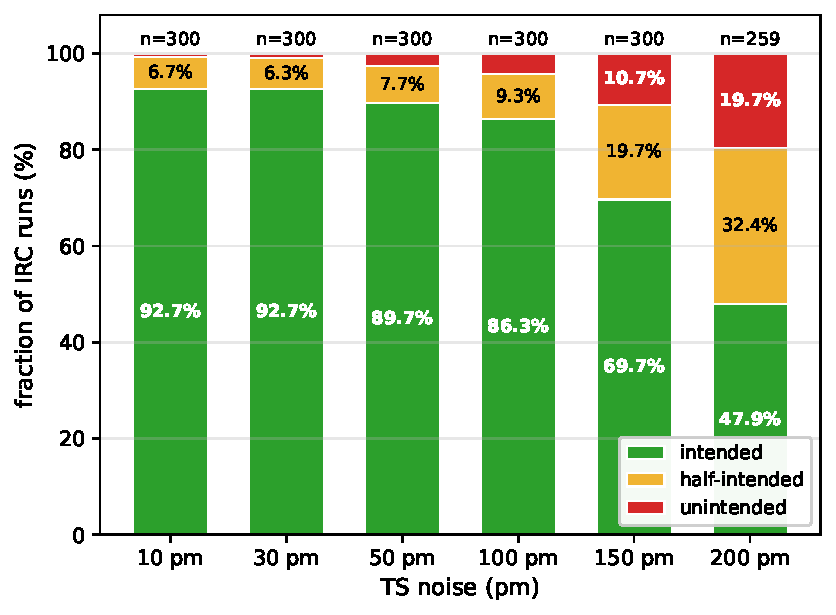
\includegraphics[width=\textwidth]{figures/fig_method_gad_eckart_irc_bars_topo.pdf}
\caption{GAD Eckart --- IRC TOPO (all endpoints)}
\end{subfigure}
\caption{\textbf{\texttt{gad\_dt003} with Eckart projection, dt=0.003, 2000 steps.}
Left: local-gate convergence rate.
Right: \texttt{sella\_hip} IRC TOPO outcome on every sample's final geometry.
Labels on bars are percentages of the 300-sample universe.}
\end{figure}

\begin{figure}[!htbp]
\centering
\begin{subfigure}[t]{0.495\textwidth}
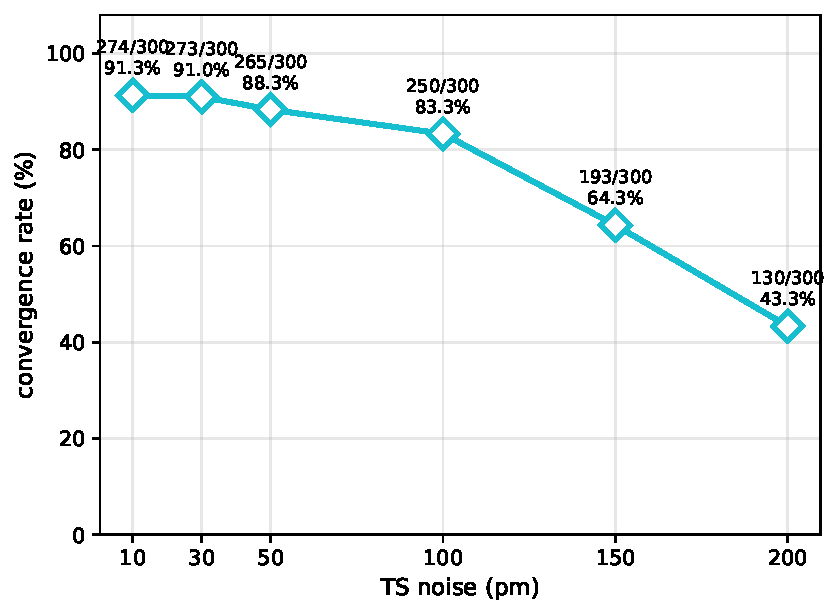
\includegraphics[width=\textwidth]{figures/fig_method_gad_no_eckart_conv_line.pdf}
\caption{GAD no-Eckart --- local gate \\($n_{\text{neg}}{=}1 \wedge f_{\max}{<}0.01$)}
\end{subfigure}
\hfill
\begin{subfigure}[t]{0.495\textwidth}
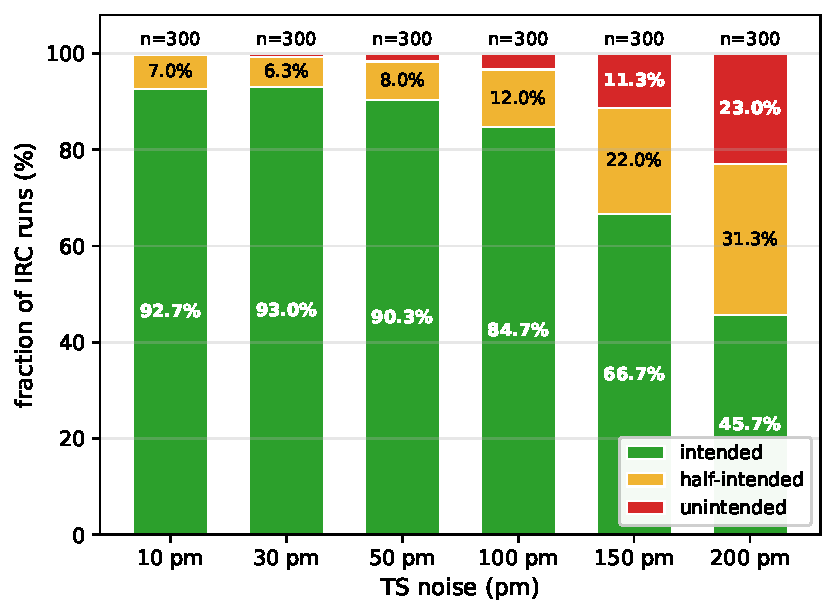
\includegraphics[width=\textwidth]{figures/fig_method_gad_no_eckart_irc_bars_topo.pdf}
\caption{GAD no-Eckart --- IRC TOPO (all endpoints)}
\end{subfigure}
\caption{\textbf{\texttt{gad\_dt003\_no\_eckart}: raw Hessian GAD, dt=0.003, 2000 steps.}
Eckart projection removed from dynamics; local gate uses fmax.}
\end{figure}

\begin{figure}[!htbp]
\centering
\begin{subfigure}[t]{0.495\textwidth}
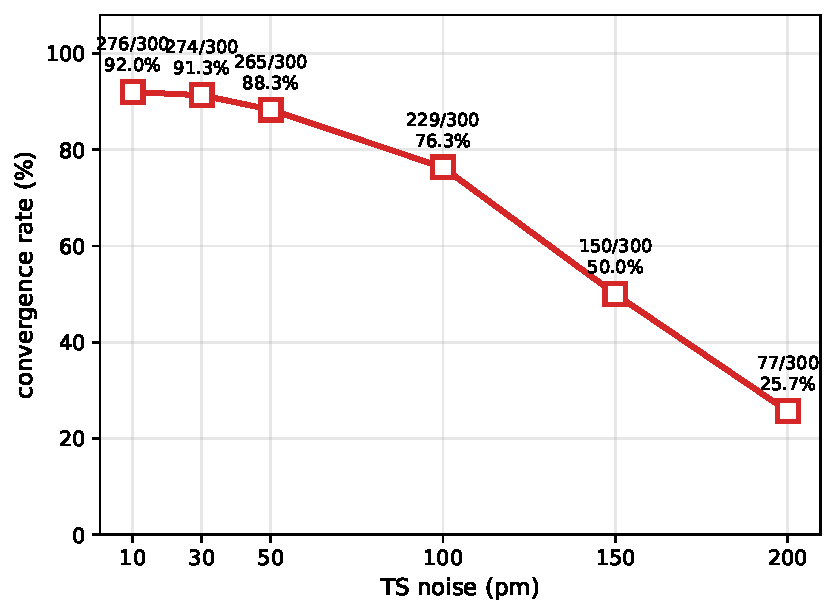
\includegraphics[width=\textwidth]{figures/fig_method_sella_carte_2k_conv_line.pdf}
\caption{Sella cart+Eckart --- local gate \\($n_{\text{neg}}{=}1 \wedge f_{\max}{<}0.01$)}
\end{subfigure}
\hfill
\begin{subfigure}[t]{0.495\textwidth}
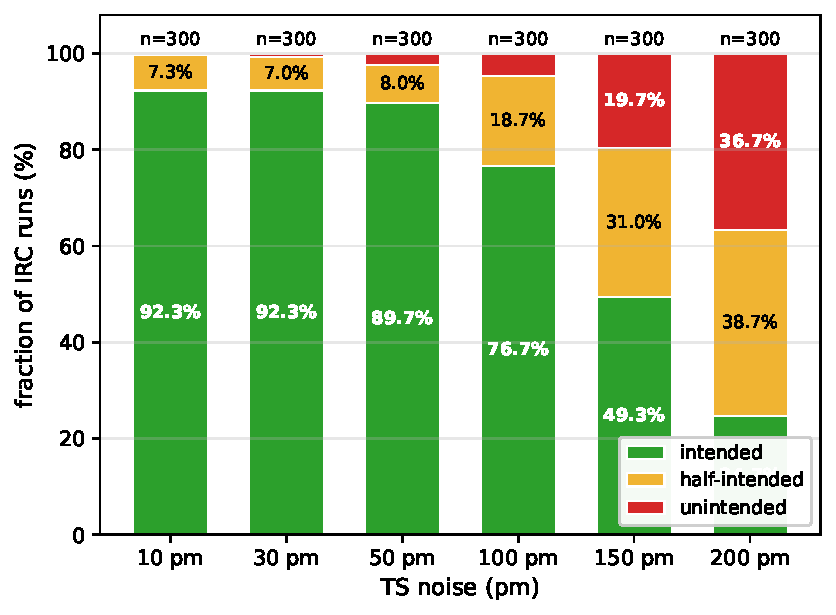
\includegraphics[width=\textwidth]{figures/fig_method_sella_carte_2k_irc_bars_topo.pdf}
\caption{Sella cart+Eckart --- IRC TOPO (all endpoints)}
\end{subfigure}
\caption{\textbf{Sella cartesian + Eckart, 2000 steps, HIP Hessian every step.}}
\end{figure}

\begin{figure}[!htbp]
\centering
\begin{subfigure}[t]{0.495\textwidth}
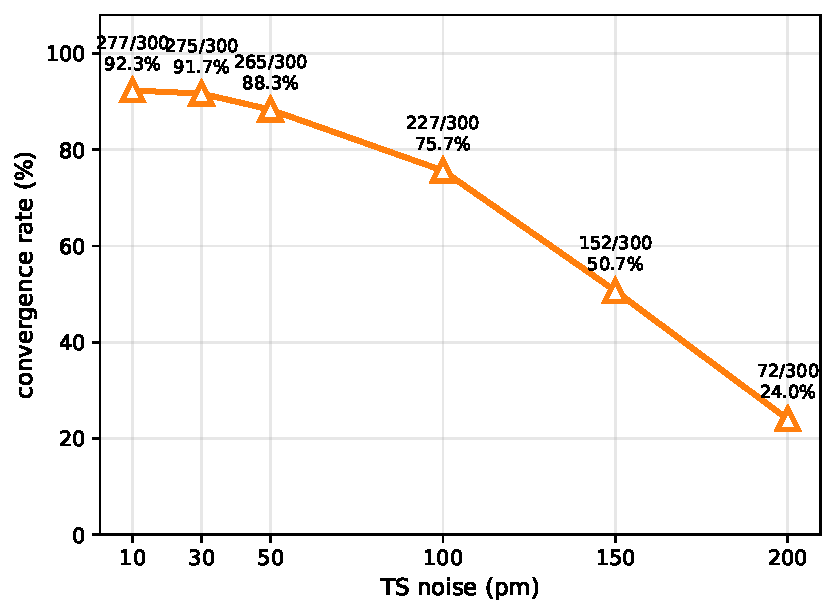
\includegraphics[width=\textwidth]{figures/fig_method_sella_cart_2k_conv_line.pdf}
\caption{Sella cart no-Eckart --- local gate}
\end{subfigure}
\hfill
\begin{subfigure}[t]{0.495\textwidth}
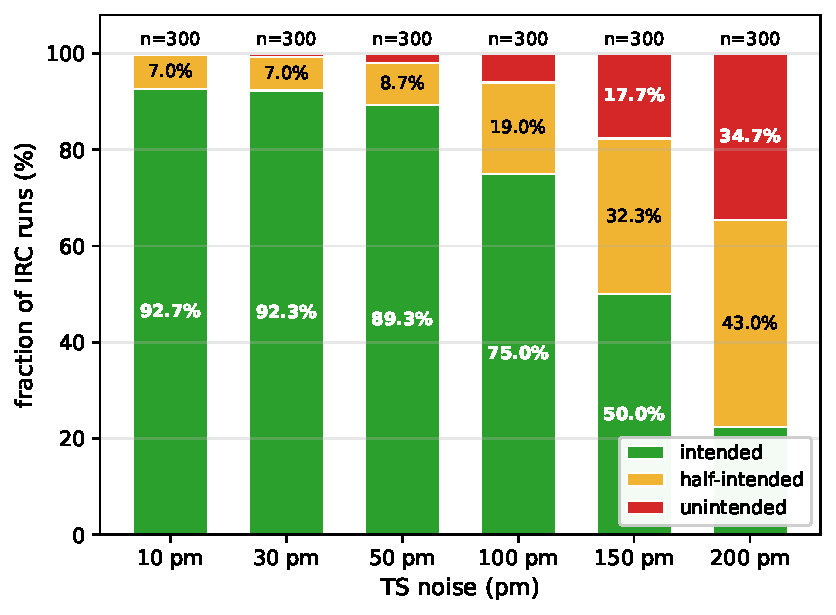
\includegraphics[width=\textwidth]{figures/fig_method_sella_cart_2k_irc_bars_topo.pdf}
\caption{Sella cart no-Eckart --- IRC TOPO (all endpoints)}
\end{subfigure}
\caption{\textbf{Sella cartesian, no Eckart, 2000 steps, HIP Hessian every step.}}
\end{figure}

\begin{figure}[!htbp]
\centering
\begin{subfigure}[t]{0.495\textwidth}
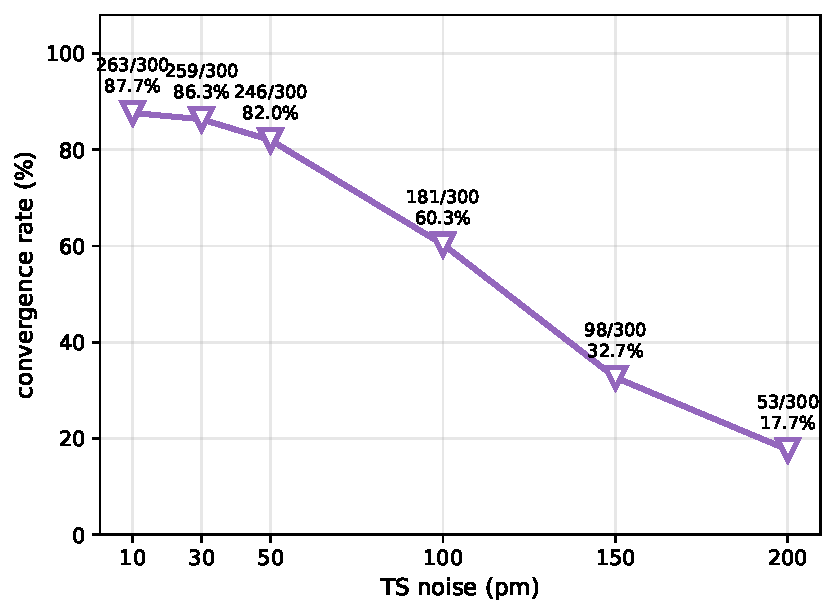
\includegraphics[width=\textwidth]{figures/fig_method_sella_int_2k_conv_line.pdf}
\caption{Sella internal --- local gate}
\end{subfigure}
\hfill
\begin{subfigure}[t]{0.495\textwidth}
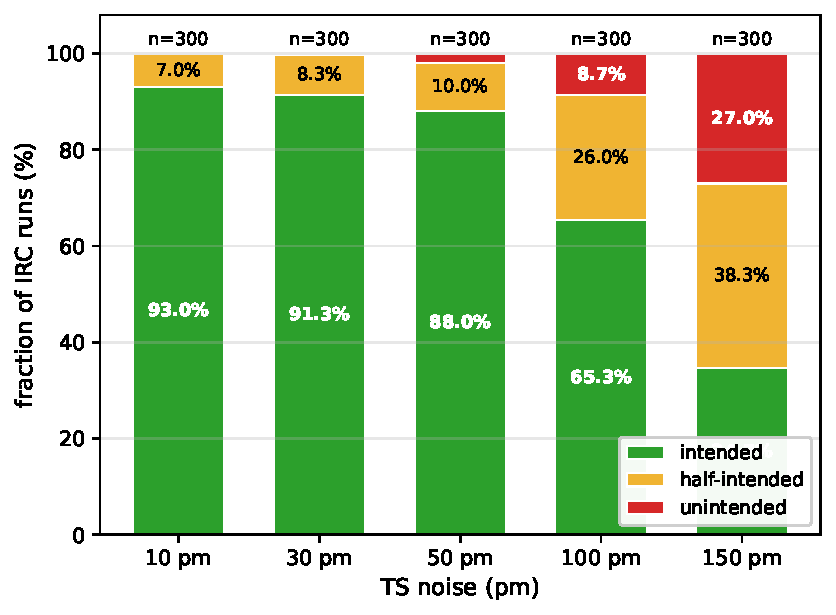
\includegraphics[width=\textwidth]{figures/fig_method_sella_int_2k_irc_bars_topo.pdf}
\caption{Sella internal --- IRC TOPO (all endpoints)}
\end{subfigure}
\caption{\textbf{Sella internal coords (no Eckart --- Sella handles DOF removal
intrinsically), 2000 steps, HIP Hessian every step.}
200\,pm IRC cell still computing at report time.}
\end{figure}

\newpage
\FloatBarrier
% =================================================================
\section{The Eckart Story (re-examined)}
\label{sec:eckart_deep}
% =================================================================

The Round~1 result was ``Eckart projection is the main unlock for GAD''.
The new data refines this: Eckart is a \textbf{step-efficiency multiplier},
not a fundamental dynamics switch. Specifically:

\begin{center}
\textbf{Median converged-step (same-sample intersection, both methods converged)} \\[0.3em]
\begin{tabular}{rccc}
\toprule
Noise & Eckart & no-Eckart & ratio \\
\midrule
10\,pm  & 94 & 125 & 1.33$\times$ \\
30\,pm  & 206 & 271 & 1.32$\times$ \\
50\,pm  & 289 & 391 & 1.35$\times$ \\
100\,pm & 453 & 607 & 1.34$\times$ \\
150\,pm & 568 & 757 & 1.33$\times$ \\
200\,pm & 678 & 842 & 1.24$\times$ \\
\bottomrule
\end{tabular}
\end{center}

\paragraph{Constant $\sim$1.33$\times$ ratio across noise.} No-Eckart
GAD needs roughly 33\% more steps to reach the same saddle on the same
starting geometry. Mechanism: the raw Cartesian Hessian has 6
near-zero TR-mode eigenvalues; the ``lowest eigenvalue'' eigenvector
occasionally leaks into TR space, and GAD wastes a fraction of each
step translating/rotating the molecule.

\paragraph{Why Round~1 looked catastrophic for no-Eckart.} Round~1 ran
\texttt{pure\_gad} at dt=0.005, 300 steps. Asking ``how many samples
of the new \texttt{gad\_dt003\_no\_eckart} run converge if truncated
at 300 steps'':

\begin{center}
\begin{tabular}{rcccc}
\toprule
Noise & full (2000 steps) & cap@300 & cap@500 & cap@1000 \\
\midrule
10\,pm  & 91.3\% & \textbf{84.3\%} & 89.0\% & 90.3\% \\
30\,pm  & 91.0\% & \textbf{52.7\%} & 81.3\% & 89.3\% \\
50\,pm  & 88.3\% & \textbf{25.7\%} & 65.3\% & 86.7\% \\
100\,pm & 83.3\% & \textbf{4.3\%}  & 30.7\% & 72.0\% \\
150\,pm & 64.3\% & \textbf{0.7\%}  & 13.3\% & 48.3\% \\
200\,pm & 43.3\% & \textbf{0.7\%}  & 6.0\%  & 27.3\% \\
\bottomrule
\end{tabular}
\end{center}

The cap@300 column is essentially what Round~1 \texttt{pure\_gad} saw.
Near-zero above 100\,pm. With an adequate 2000-step budget the same
dynamics reaches 43\% at 200\,pm.

\paragraph{Corrected narrative.} Eckart gives GAD a 1.33$\times$ step
efficiency. Under \emph{tight} budget (300 steps) this is the difference
between finishing and timing out, so Eckart looked essential. Under
\emph{adequate} budget (2000 steps) it's a 3--9\,pp bump, and IRC-level
outcomes are within 0--3\,pp of the Eckart variant. The useful framing
is \textbf{``projected dynamics + enough steps''}, not ``Eckart is
magic''.

\newpage
\FloatBarrier
% =================================================================
\section{Gate vs IRC Sample Overlap}
% =================================================================

For each method and noise level, every sample falls into one of four
quadrants: \{local gate pass, IRC TOPO pass\}. This quantifies whether
a method's ``converged'' label agrees with IRC's verdict.

\begin{figure}[!htbp]
\centering
\begin{subfigure}[t]{0.48\textwidth}
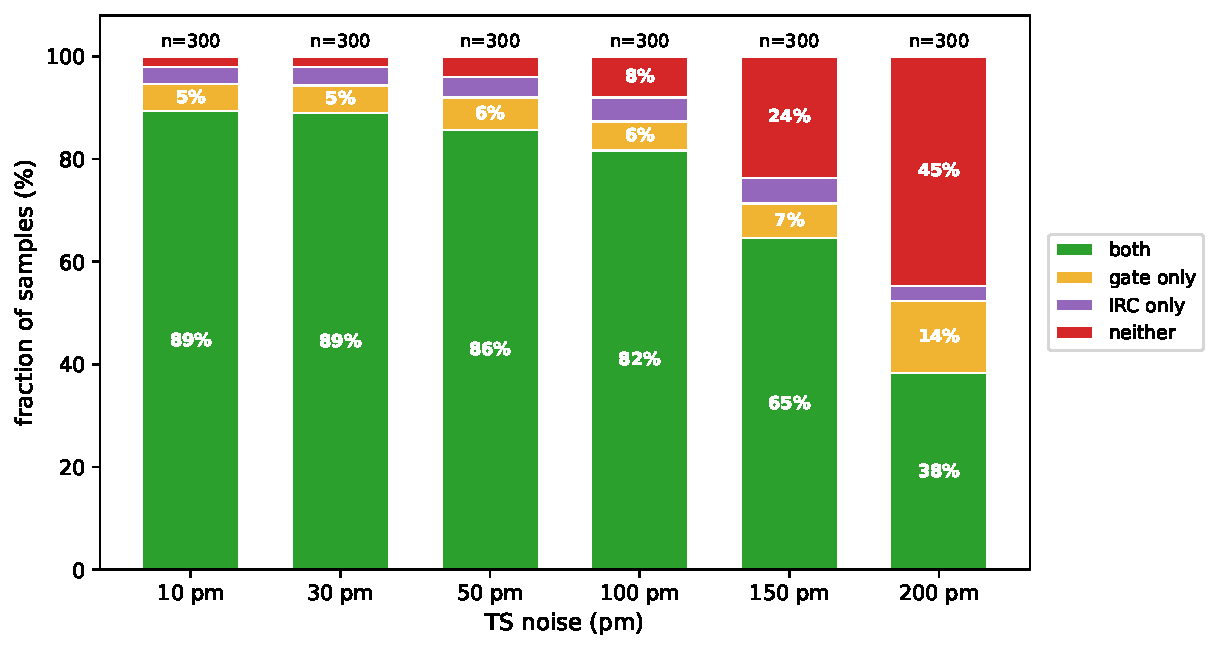
\includegraphics[width=\textwidth]{figures/fig_gate_vs_irc_gad_eckart.pdf}
\caption{GAD Eckart}
\end{subfigure}
\hfill
\begin{subfigure}[t]{0.48\textwidth}
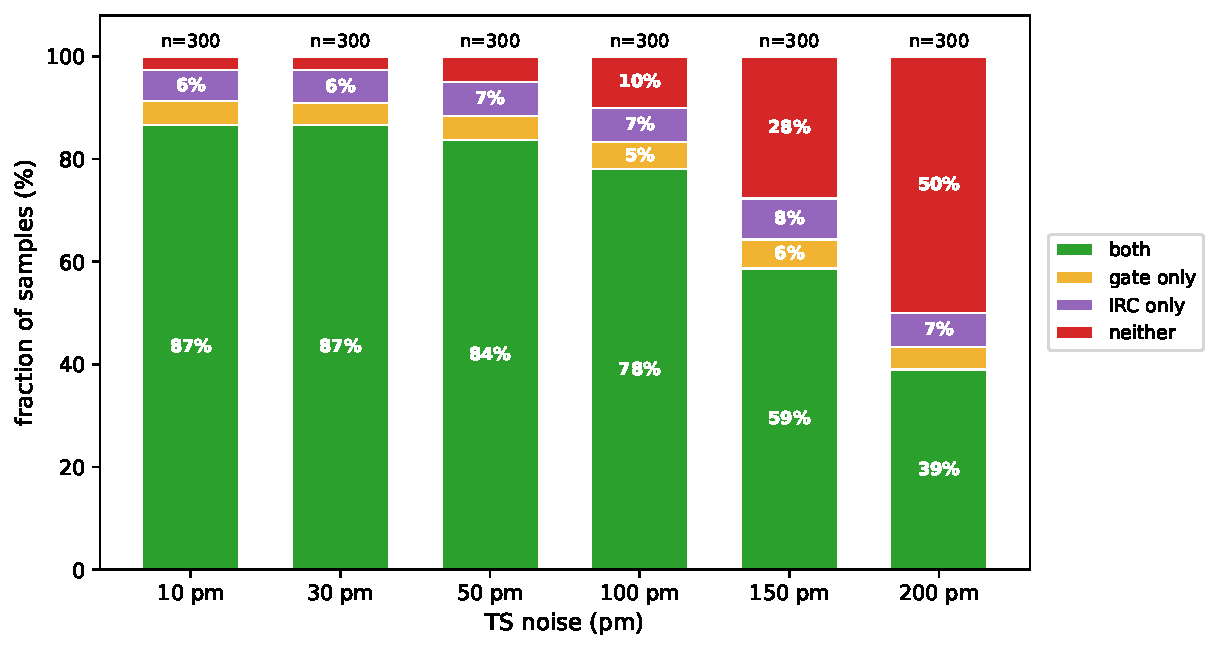
\includegraphics[width=\textwidth]{figures/fig_gate_vs_irc_gad_no_eckart.pdf}
\caption{GAD no-Eckart}
\end{subfigure}
\vskip0.5em
\begin{subfigure}[t]{0.48\textwidth}
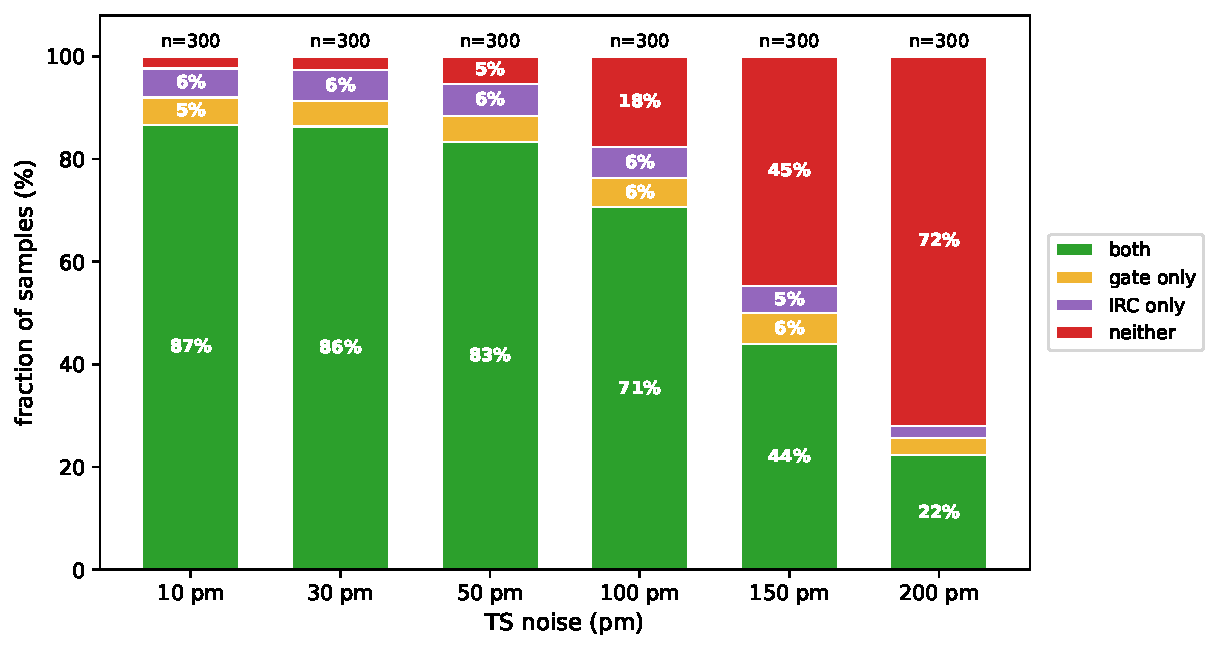
\includegraphics[width=\textwidth]{figures/fig_gate_vs_irc_sella_carte_2k.pdf}
\caption{Sella cart+Eckart}
\end{subfigure}
\hfill
\begin{subfigure}[t]{0.48\textwidth}
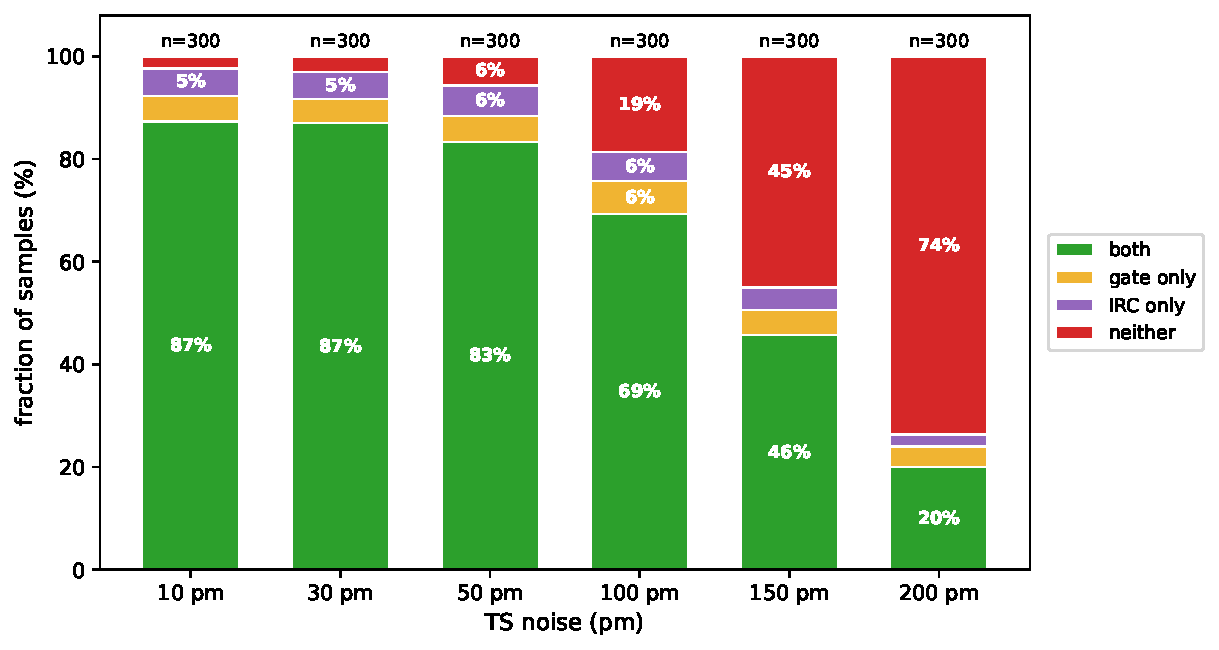
\includegraphics[width=\textwidth]{figures/fig_gate_vs_irc_sella_cart_2k.pdf}
\caption{Sella cart no-Eckart}
\end{subfigure}
\vskip0.5em
\begin{subfigure}[t]{0.48\textwidth}
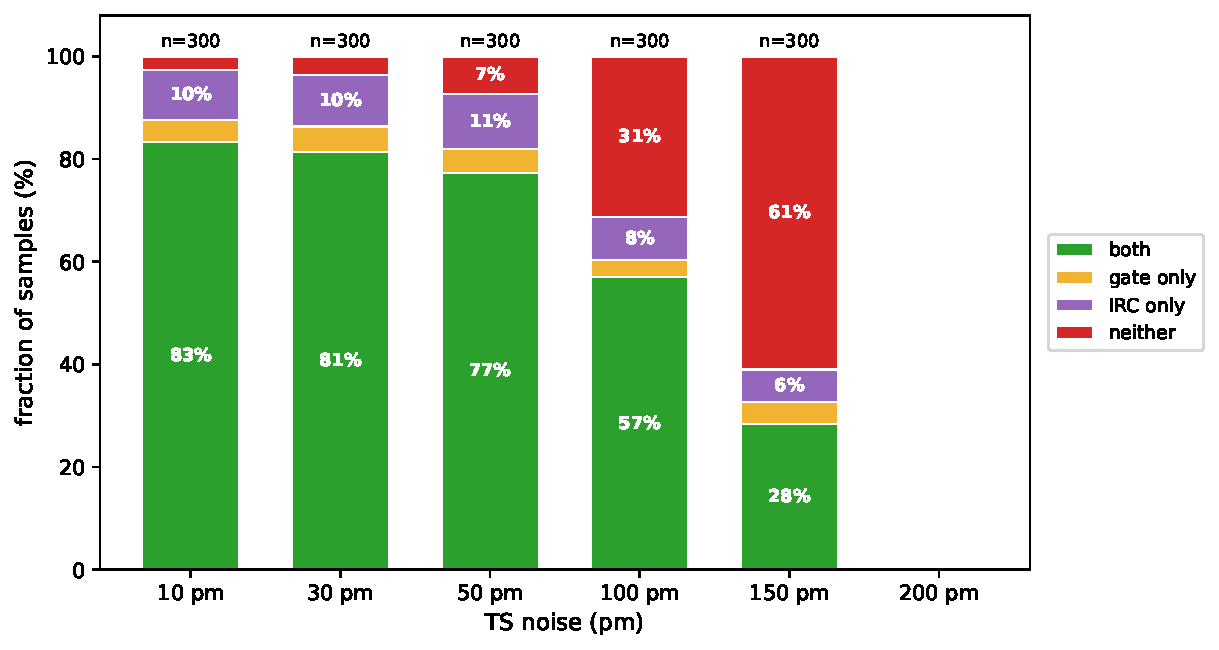
\includegraphics[width=\textwidth]{figures/fig_gate_vs_irc_sella_int_2k.pdf}
\caption{Sella internal}
\end{subfigure}
\caption{\textbf{Per-method gate vs.\ IRC-TOPO overlap, all 5 methods.}
Green (``both''): gate-converged AND IRC-TOPO passes. Yellow
(``gate only''): gate says converged, IRC disagrees (over-claim by
local gate). Purple (``IRC only''): gate says failed, IRC says
chemically correct (under-claim by local gate). Red (``neither''):
both agree the sample failed. The red region grows sharply with noise
for Sella and internal; stays small for GAD.}
\end{figure}

\newpage
\FloatBarrier
% =================================================================
\section{Compute Costs}
% =================================================================

\begin{center}
\textbf{Median wall time per sample (s)} \\[0.3em]
\begin{tabular}{l|cccccc}
\toprule
Method & 10\,pm & 30\,pm & 50\,pm & 100\,pm & 150\,pm & 200\,pm \\
\midrule
GAD Eckart                  & 3.9 & 7.3 & 13.7 & 23.9 & 51.5 & 86.1 \\
GAD no-Eckart               & 6.9 & 10.3 & 16.5 & 24.9 & 49.5 & 80.0 \\
Sella cart+Eckart           & 2.3 & 3.7 & 6.3 & 16.4 & 58.9 & 113.2 \\
Sella cart no-Eckart        & 2.2 & 3.5 & 6.2 & 17.2 & 55.0 & 119.6 \\
Sella internal              & 4.3 & 5.6 & 10.3 & 46.7 & 117.4 & 151.7 \\
\bottomrule
\end{tabular}
\end{center}

\begin{center}
\textbf{Valid TSs per GPU-hour (local gate)} \\[0.3em]
\begin{tabular}{l|cccccc}
\toprule
Method & 10\,pm & 30\,pm & 50\,pm & 100\,pm & 150\,pm & 200\,pm \\
\midrule
GAD Eckart                  & 227 & 158 & 115 & 70 & 40 & 22 \\
GAD no-Eckart               & 168 & 115 & 84 & 56 & 30 & 16.5 \\
Sella cart+Eckart           & \textbf{264} & \textbf{249} & \textbf{175} & 79 & 24 & 8.6 \\
Sella cart no-Eckart        & 267 & 252 & 177 & 75 & 26 & 7.7 \\
Sella internal              & 148 & 116 & 84 & 31 & 10 & 4 \\
\bottomrule
\end{tabular}
\end{center}

Crossover is at $\sim$100\,pm. Below: Sella cartesian is fastest source
of valid TSs. Above: GAD --- the Sella convergence-rate collapse
dominates per-hour yield.

\newpage
% =================================================================
\section{Appendix}
% =================================================================

\FloatBarrier
\subsection{Per-method bar charts: RMSD and endpoint vibrational quality}

Three criteria per method: TOPO (already shown in §2.2), strict RMSD
($<0.3$\,\AA), endpoint vibrational quality (both / one / neither at
vibrational minimum).

\begin{figure}[!htbp]
\centering
\begin{subfigure}[t]{0.48\textwidth}
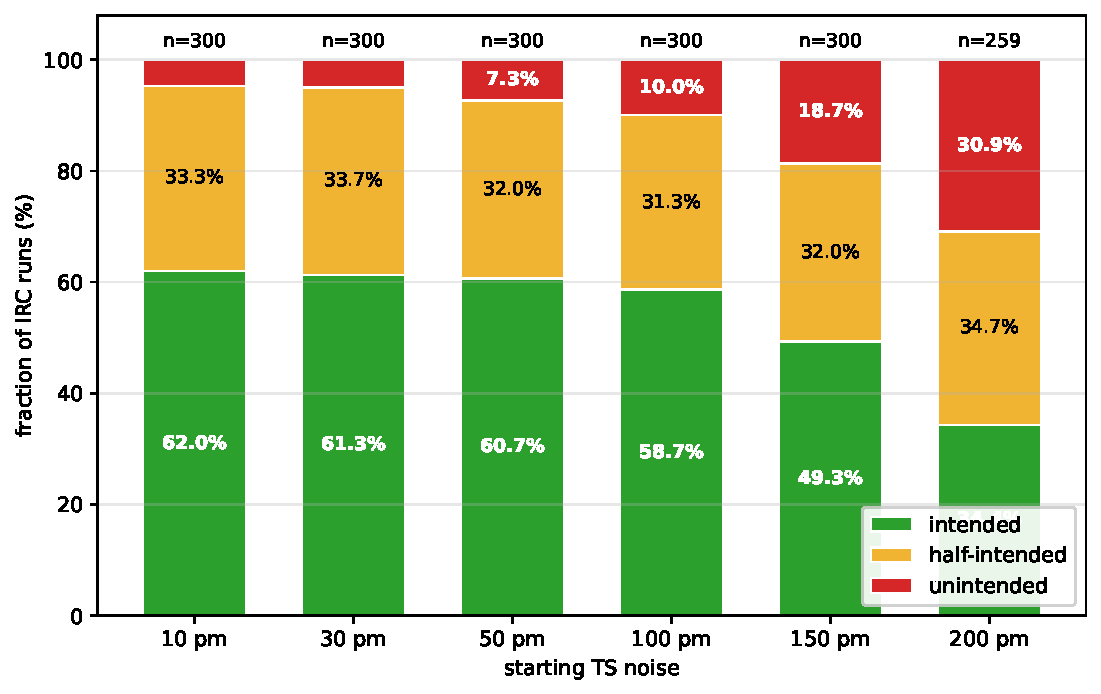
\includegraphics[width=\textwidth]{figures/fig_sella_allep_bars_rmsd.pdf}
\caption{GAD Eckart, RMSD}
\end{subfigure}
\hfill
\begin{subfigure}[t]{0.48\textwidth}
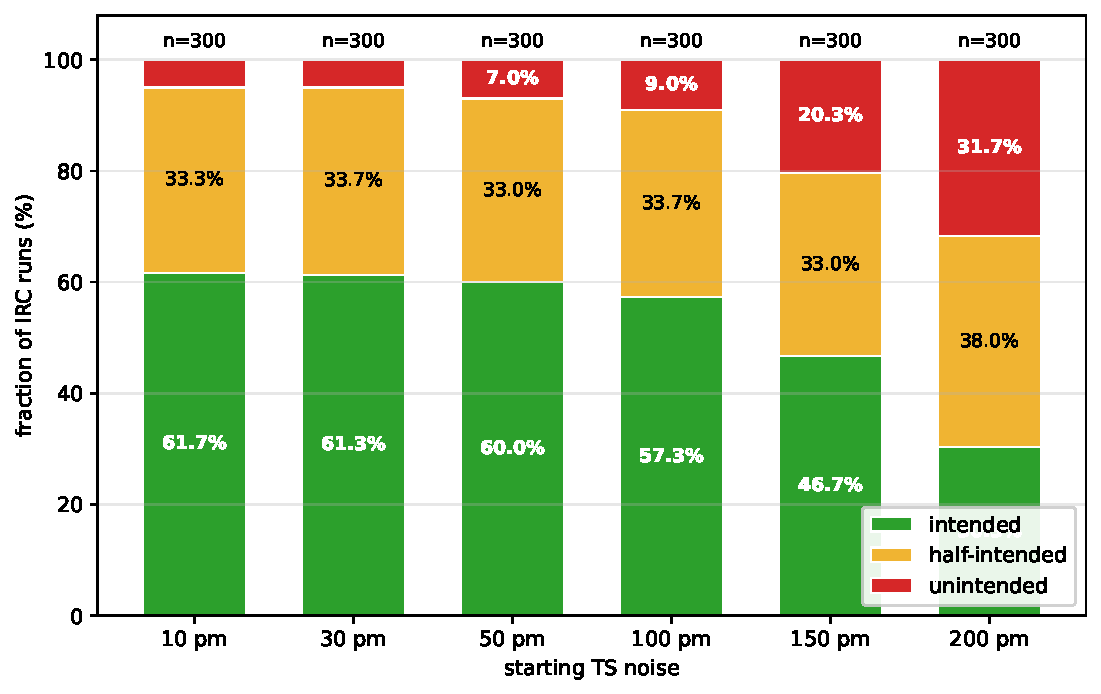
\includegraphics[width=\textwidth]{figures/fig_gad_noeck_new_bars_rmsd.pdf}
\caption{GAD no-Eckart, RMSD}
\end{subfigure}
\vskip0.5em
\begin{subfigure}[t]{0.48\textwidth}
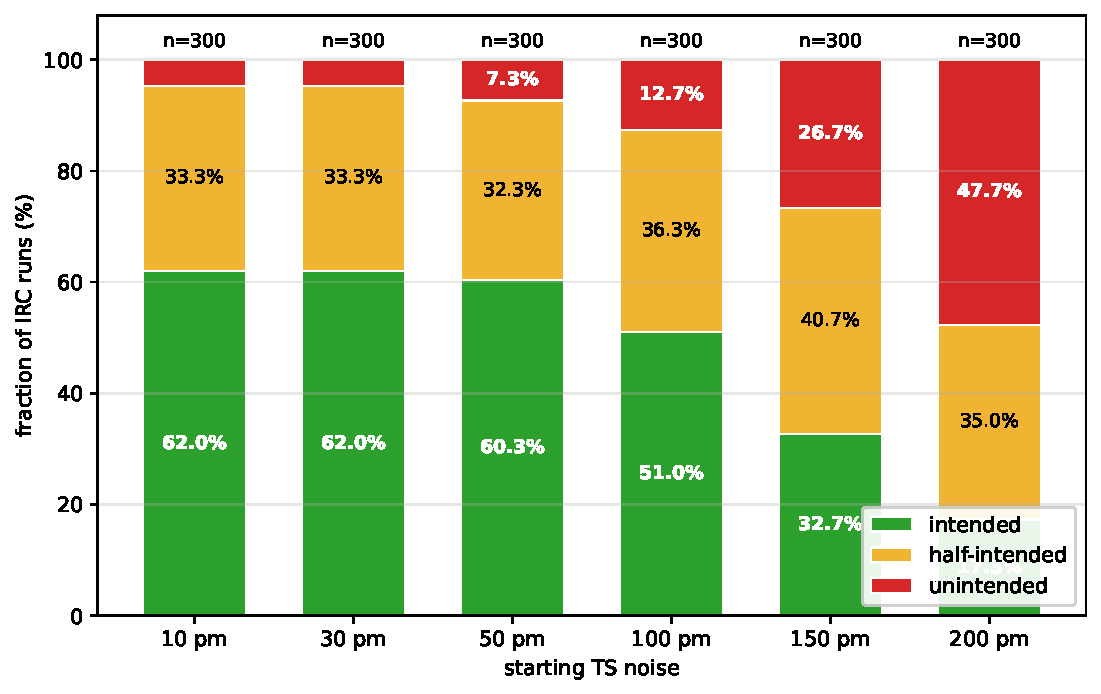
\includegraphics[width=\textwidth]{figures/fig_sella_carte_2k_bars_rmsd.pdf}
\caption{Sella cart+Eckart, RMSD}
\end{subfigure}
\hfill
\begin{subfigure}[t]{0.48\textwidth}
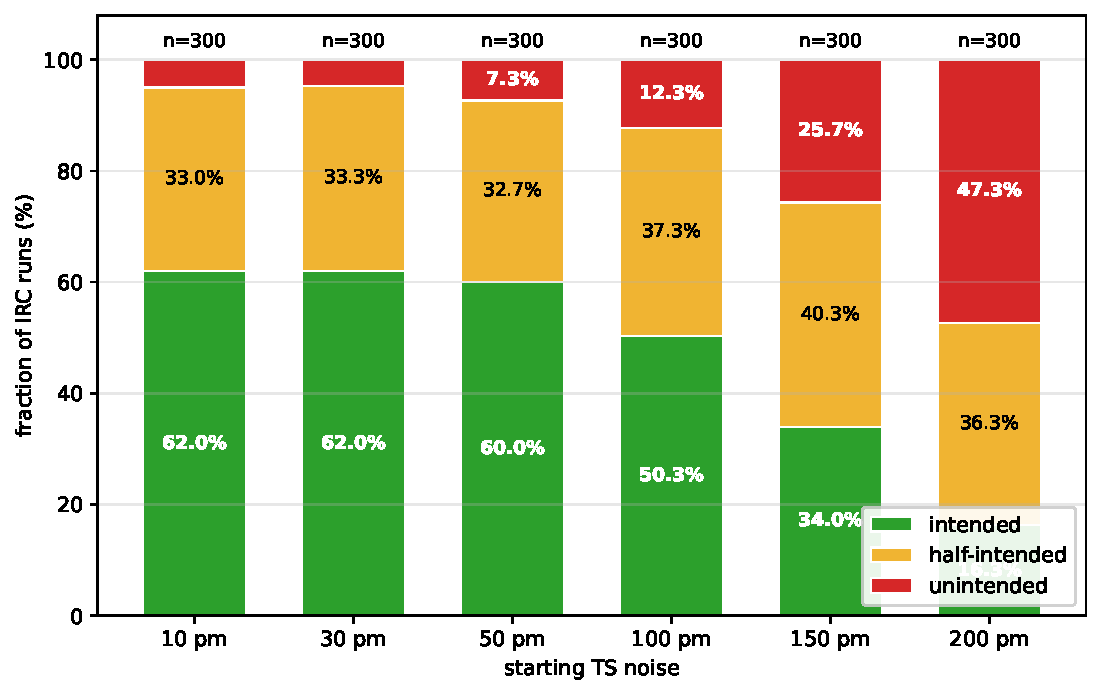
\includegraphics[width=\textwidth]{figures/fig_sella_cart_2k_bars_rmsd.pdf}
\caption{Sella cart no-Eckart, RMSD}
\end{subfigure}
\vskip0.5em
\begin{subfigure}[t]{0.48\textwidth}
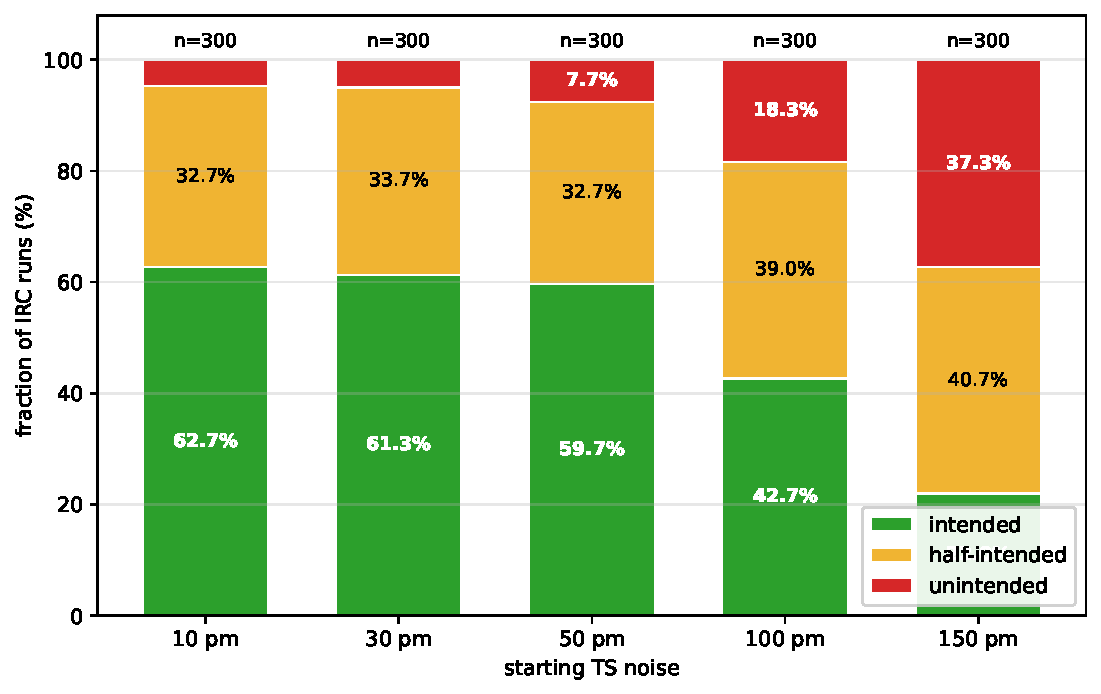
\includegraphics[width=\textwidth]{figures/fig_sella_int_2k_bars_rmsd.pdf}
\caption{Sella internal, RMSD}
\end{subfigure}
\caption{\textbf{Strict RMSD criterion ($<0.3$\,\AA) per method.}
Denominator = 300 samples per cell.}
\end{figure}

\begin{figure}[!htbp]
\centering
\begin{subfigure}[t]{0.48\textwidth}
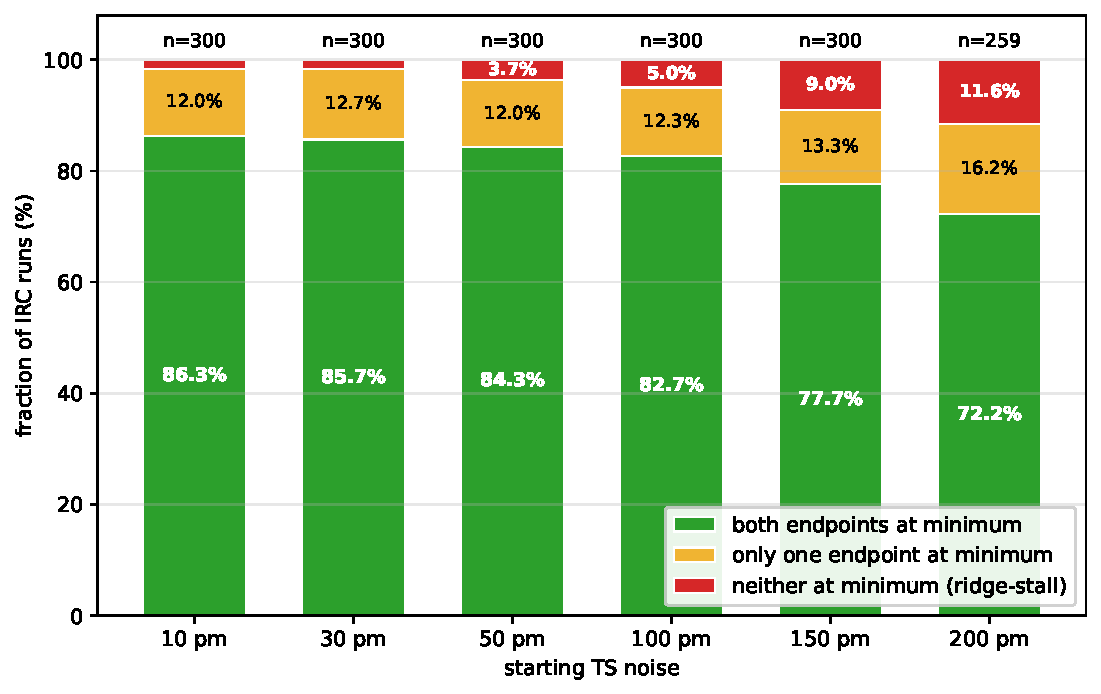
\includegraphics[width=\textwidth]{figures/fig_sella_allep_bars_endpoint.pdf}
\caption{GAD Eckart}
\end{subfigure}
\hfill
\begin{subfigure}[t]{0.48\textwidth}
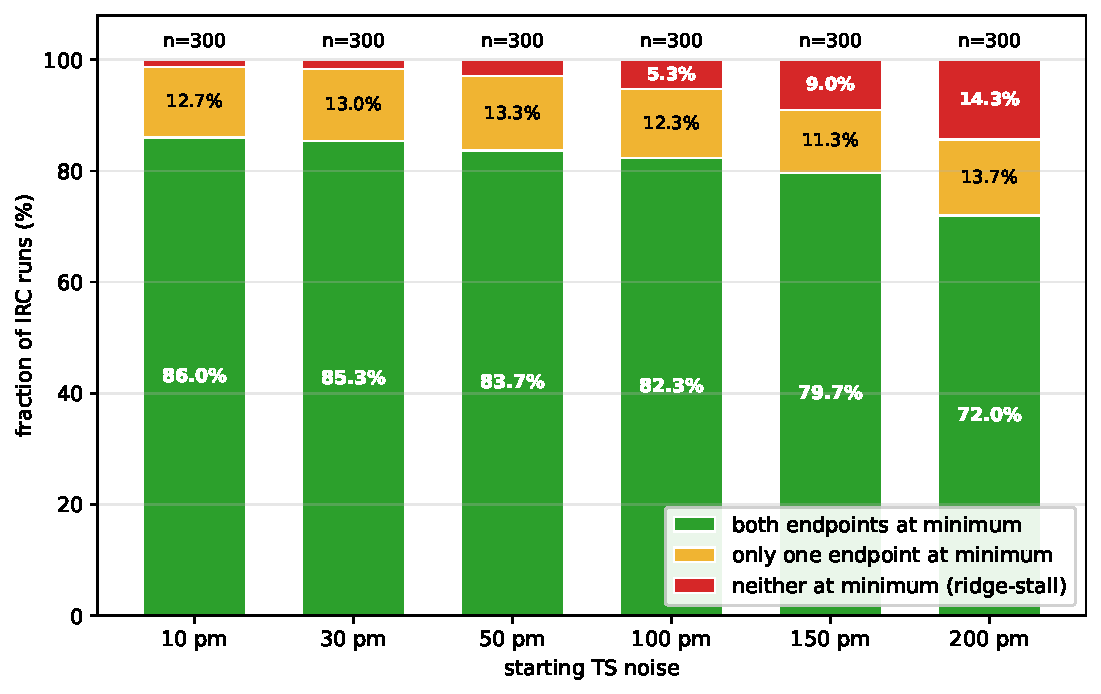
\includegraphics[width=\textwidth]{figures/fig_gad_noeck_new_bars_endpoint.pdf}
\caption{GAD no-Eckart}
\end{subfigure}
\vskip0.5em
\begin{subfigure}[t]{0.48\textwidth}
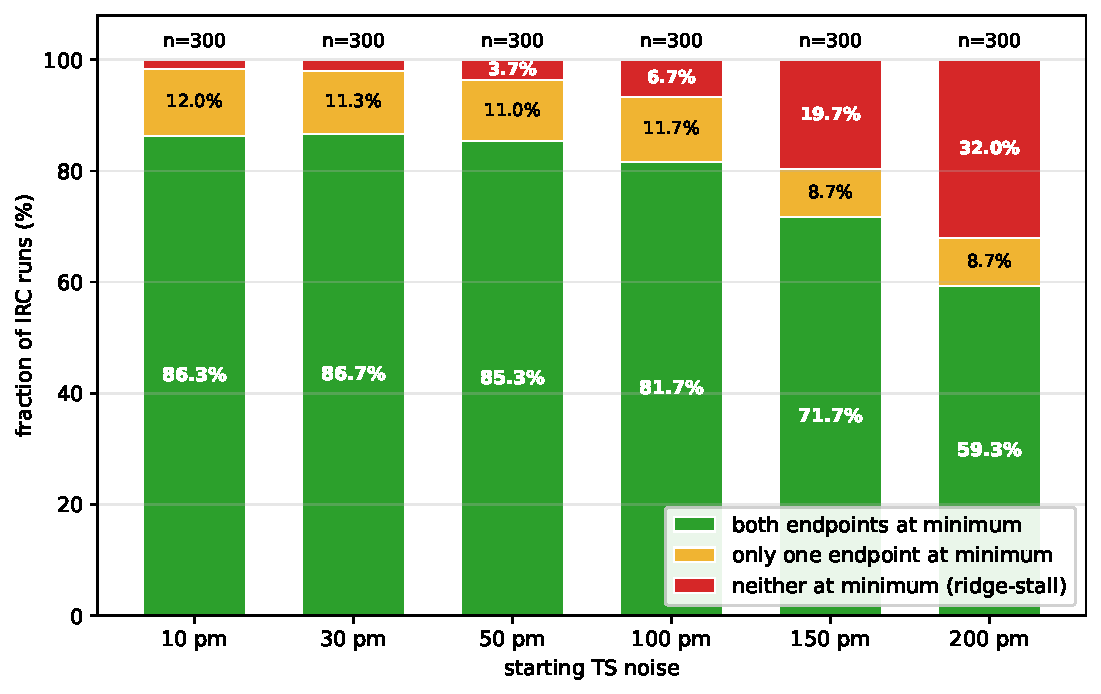
\includegraphics[width=\textwidth]{figures/fig_sella_carte_2k_bars_endpoint.pdf}
\caption{Sella cart+Eckart}
\end{subfigure}
\hfill
\begin{subfigure}[t]{0.48\textwidth}
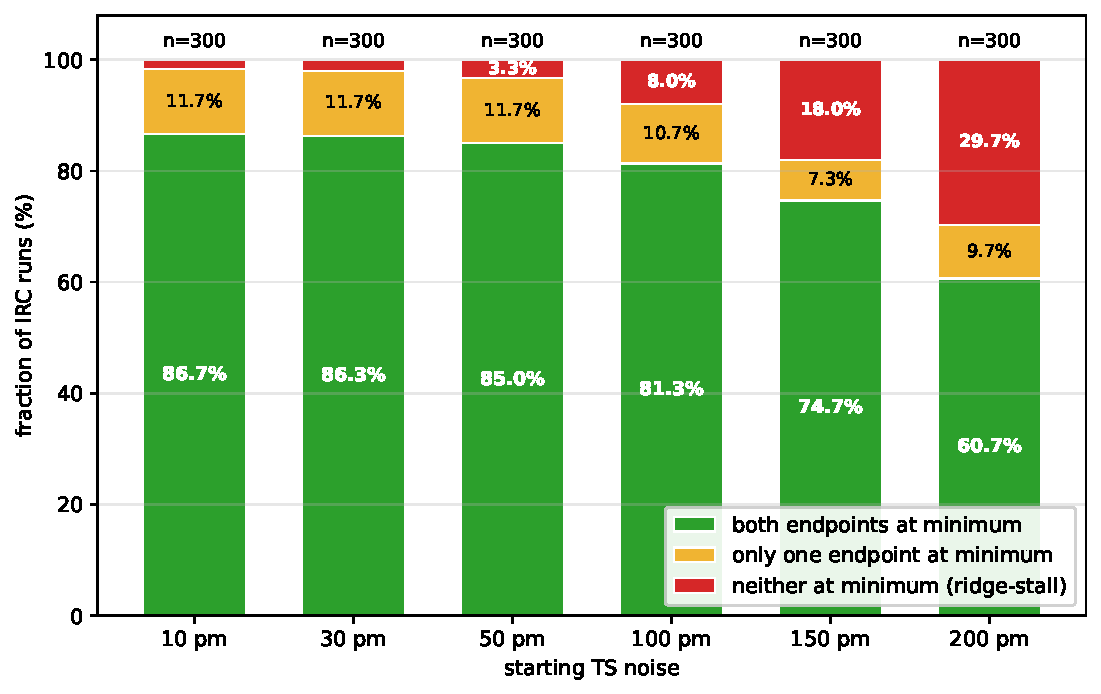
\includegraphics[width=\textwidth]{figures/fig_sella_cart_2k_bars_endpoint.pdf}
\caption{Sella cart no-Eckart}
\end{subfigure}
\vskip0.5em
\begin{subfigure}[t]{0.48\textwidth}
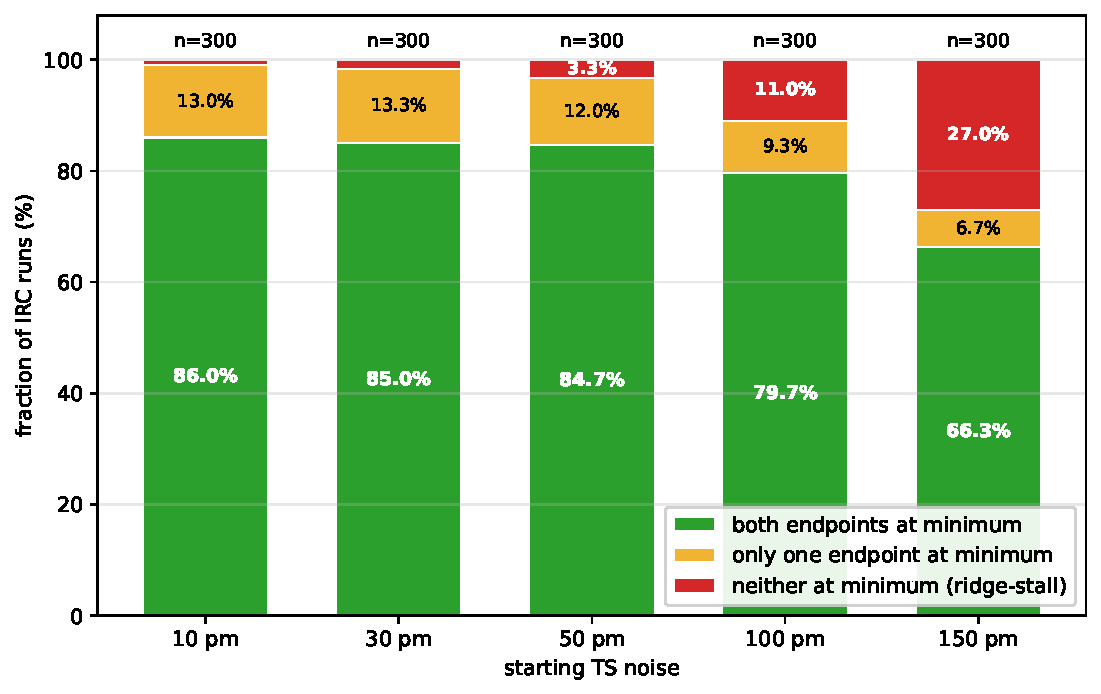
\includegraphics[width=\textwidth]{figures/fig_sella_int_2k_bars_endpoint.pdf}
\caption{Sella internal}
\end{subfigure}
\caption{\textbf{Endpoint vibrational quality per method.} Both / one /
neither IRC endpoint reaches a true minimum
($n_{\text{neg,vib}}{=}0$ on Eckart-projected Hessian).}
\end{figure}

\newpage
\FloatBarrier
\subsection{All-three-classes line charts (cluttered, appendix only)}

The main narrative uses ``intended only'' lines for readability. For
completeness, the ``intended + half + unintended'' breakdown per method:

\begin{figure}[!htbp]
\centering
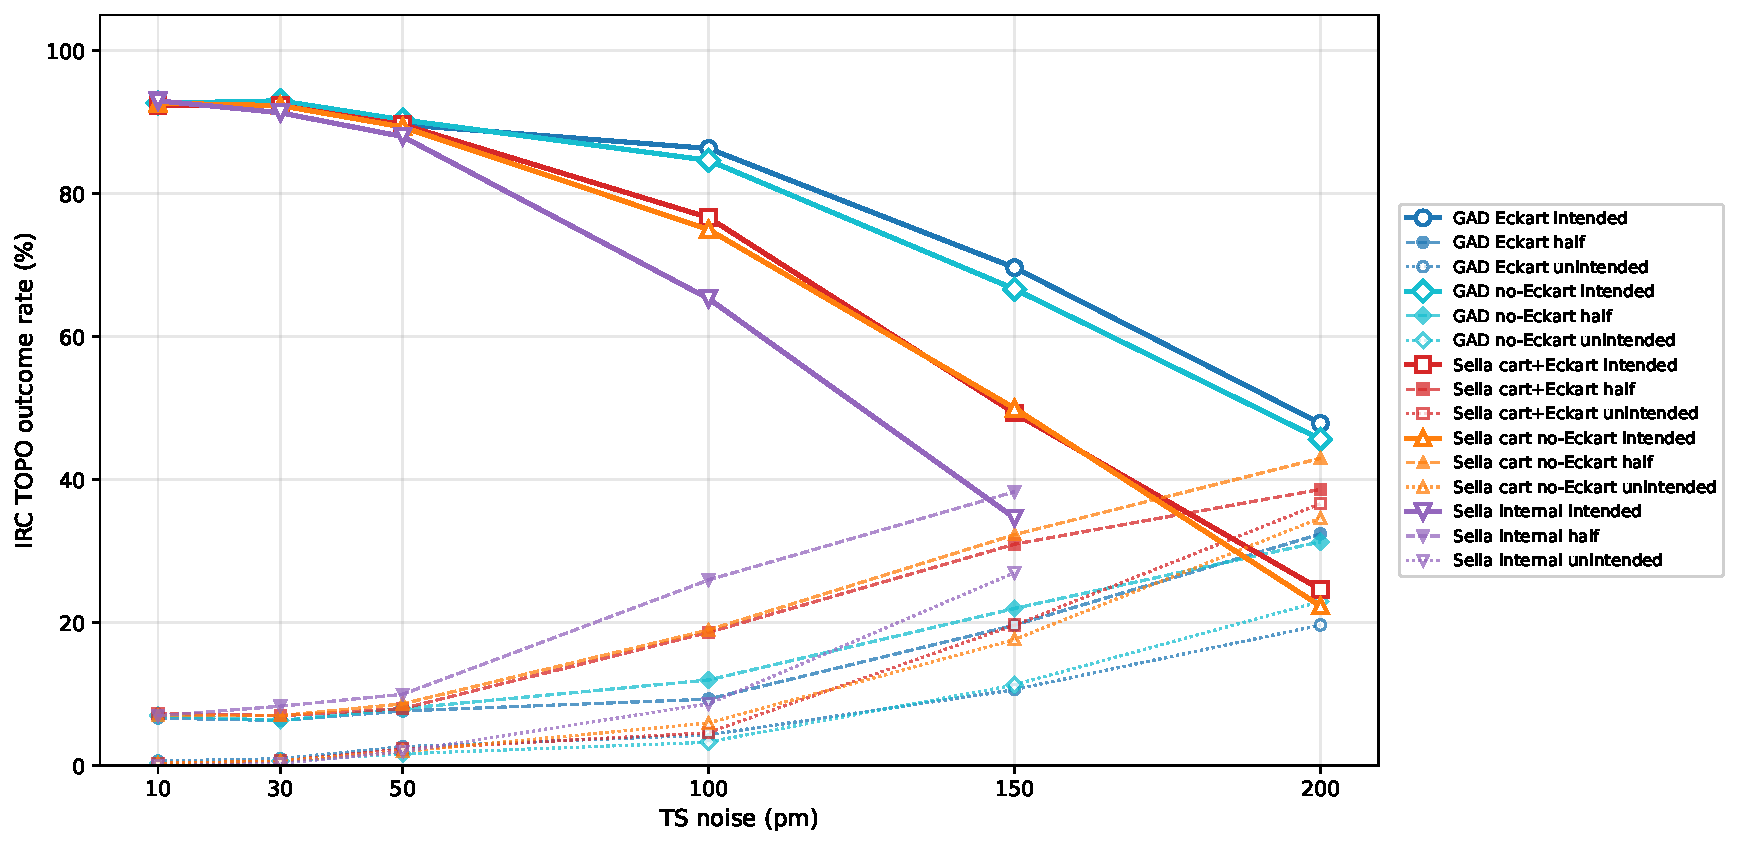
\includegraphics[width=0.95\textwidth]{figures/fig_cmp_irc_topo_all_classes_5methods.pdf}
\caption{\textbf{IRC TOPO outcomes --- all three classes, all five
methods.} 15 lines total: solid = intended, dashed = half-intended,
dotted = unintended. Cluttered on purpose; see §2.1 for the uncluttered
headline view.}
\end{figure}

\begin{figure}[!htbp]
\centering
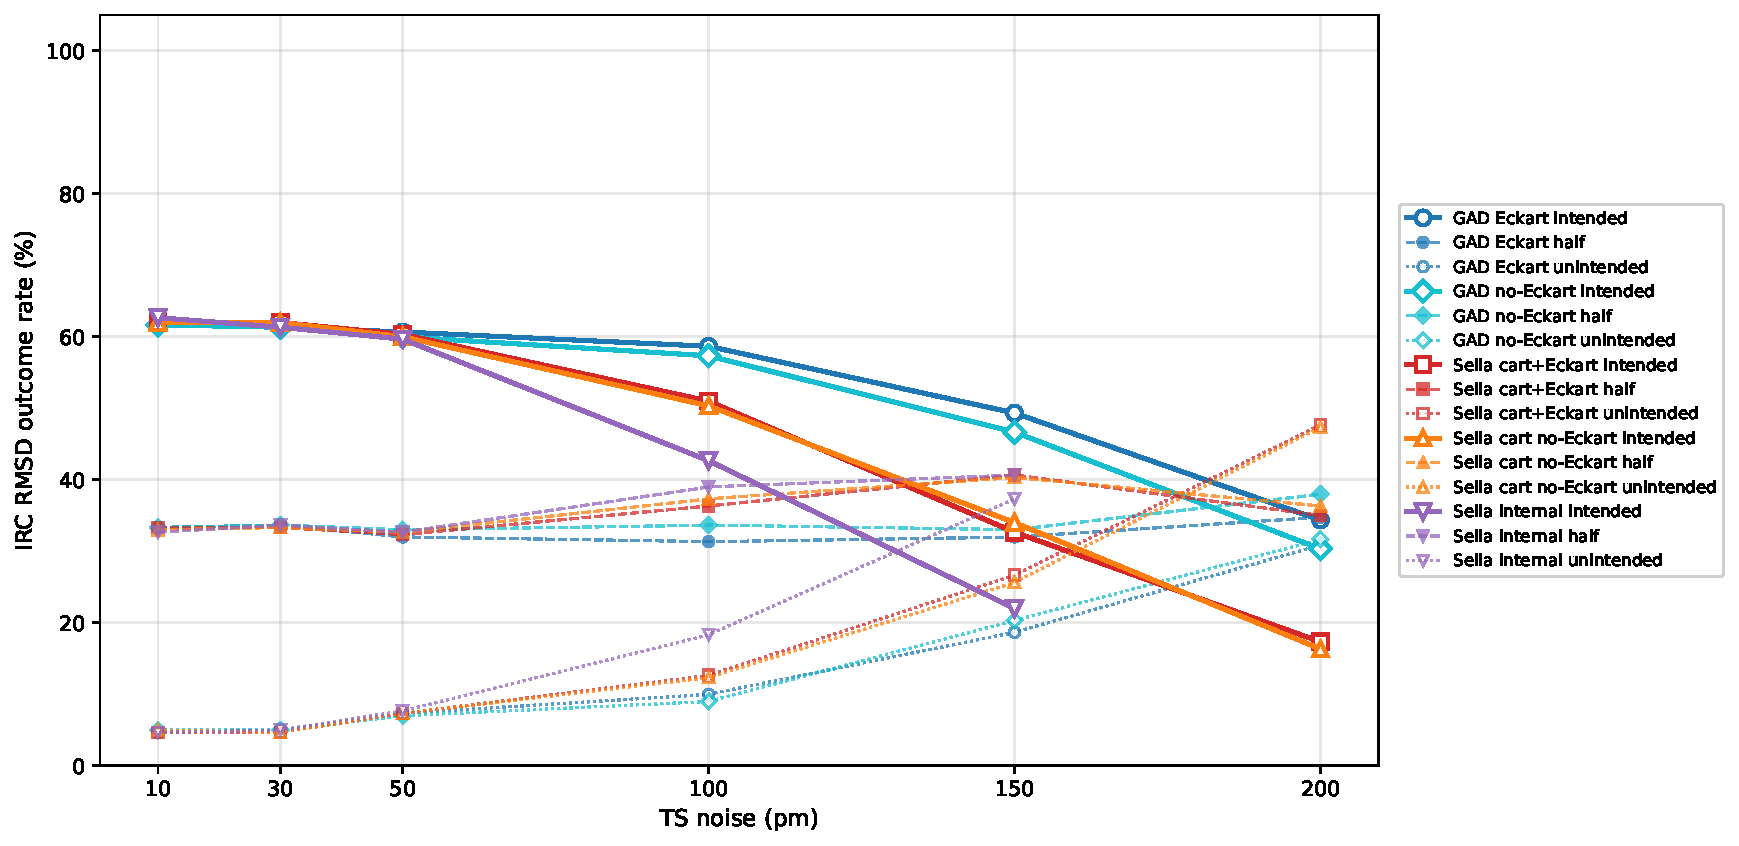
\includegraphics[width=0.95\textwidth]{figures/fig_cmp_irc_rmsd_all_classes_5methods.pdf}
\caption{\textbf{IRC strict-RMSD outcomes --- all three classes, all
five methods.} Same layout, RMSD criterion ($<0.3$\,\AA).}
\end{figure}

\FloatBarrier
\subsection{Sella IRC halt-at-step-0 fix}

Initial Sella$\to$IRC runs on Sella-refined TSs returned trivial
results (IRC halted at step 0, wall $\approx$0.24\,s per sample). Root
cause: ASE's \texttt{Optimizer.irun} checks \texttt{gradient\_converged}
before any \texttt{step()}, and Sella's IRC halt threshold (fmax$<$0.01)
matches Sella's TS optimizer threshold exactly. So a Sella-refined TS
trivially satisfied the halt before the first kick.

Fix: \texttt{src/gadplus/search/irc\_sella\_hip.py::\_force\_first\_kick}
monkey-patches \texttt{converged}, \texttt{gradient\_converged}, and
\texttt{step} so the first convergence check always returns False.
Post-first-step behavior is unchanged.

\subsection{Data locations}

\begin{center}
\begin{tabular}{ll}
\toprule
Artifact & Path \\
\midrule
GAD dt003 (Eckart) summaries & \texttt{runs/round2}, \texttt{round3} (200\,pm refilled) \\
GAD no-Eckart summaries      & \texttt{runs/gad\_no\_eckart/} \\
Sella 2000-step (3 configs)  & \texttt{runs/sella\_2000/} \\
IRC on GAD Eckart            & \texttt{runs/irc\_sellahip\_allendpoints/} \\
IRC on GAD no-Eckart         & \texttt{runs/irc\_gad\_no\_eckart/} \\
IRC on Sella cart+Eck 2000   & \texttt{runs/irc\_sella\_carte\_2000/} \\
IRC on Sella cart 2000       & \texttt{runs/irc\_sella\_cart\_2000/} \\
IRC on Sella internal 2000   & \texttt{runs/irc\_sella\_int\_2000/} \\
Figures                      & \texttt{figures/} \\
This report                  & \texttt{IRC\_COMPREHENSIVE\_2026-04-20.tex/pdf} \\
\bottomrule
\end{tabular}
\end{center}

\subsection{Open items}

\begin{itemize}[nosep,leftmargin=1.5em]
\item Sella internal 200\,pm IRC (final cell of the 5$\times$6 matrix) still
      computing at report time.
\item Rigorous predictor-corrector IRC sits at $\sim$52\% TOPO regardless
      of noise (on GAD Eckart converged TSs). Backburner for investigation.
\item Potential backfill of GAD Eckart numbers under $f_{\max}{<}0.01$ gate
      for strict apples-to-apples comparison (currently uses $\|\mathbf{F}\|_{\text{mean}}$).
\end{itemize}

\end{document}
